\documentclass{article}
%\usepackage[utf8]{inputenc}
\usepackage[utf8]{inputenc}
\usepackage[T1]{fontenc}

\usepackage[english]{babel}
\usepackage{amssymb}
\usepackage{amsmath}
\usepackage{graphicx}
\usepackage{float}
%\usepackage{caption}
%\captionsetup[figure]{font=small}
\usepackage[margin=1in]{geometry}
\usepackage{natbib}
\bibliographystyle{unsrtnat}

% Paragraphs
% Don't indent paragraphs
\setlength{\parindent}{0ex}
% Space after paragraph
\setlength{\parskip}{1em}

\title{\Large{\textbf{Methods of Computing Magnetic Field for MHD based magnetosphere simulations}}}
\author{Gary}
\date{\today}

%% use macros
\newcommand\B{\mathbf{B}}
\newcommand\J{\mathbf{J}}
\newcommand\x{\mathbf{x}}
\newcommand\M{\mathcal{M}}
\newcommand\G{\mathcal{G}}
\newcommand\I{\mathcal{I}}
\newcommand\Out{\mathcal{O}}
\newcommand\n{\mathbf{\hat{n}}}

\newcommand\sm[1]{C_{#1}}
\newcommand\vsm[1]{\mathbf{C}_{#1}}

\newcommand\GcupM{\G \cup \M}

\newcommand\ifpi{\frac{1}{4\pi}}

\newcommand\dive[1]{\boldsymbol{\nabla} \boldsymbol{\cdot} #1}
\newcommand\curl[1]{\boldsymbol{\nabla} \times #1}

\newcommand\normal[1]{\mathbf{\hat{n}}_{#1}}

\newcommand\dV{\mathrm{d}^3x}

\newcommand\xoverx{\frac{\phantom{|} \x_0-\x \phantom{|^3}}{| \x_0-\x |^3}}

\newcommand\surf[2]{\frac{1}{|\x_0-\x|^3} \Big[(\x_0-\x) (#2 \boldsymbol{\cdot} #1) + (\x_0-\x)\times (#2 \times #1) \Big]}

%% macros of macros
\newcommand\coulombInt[1]{\ifpi \int_{#1} \dive{\B}(\x) \xoverx \dV}
\newcommand\coulombIntTilde[1]{\ifpi \int_{#1} \dive{\tilde{\B}}(\x) \xoverx \dV}

\newcommand\biotsavInt[1]{\ifpi \int_{#1} \big[ \curl{\B}(\x) \big] \times \xoverx \dV}
\newcommand\biotsavIntTilde[1]{\ifpi \int_{#1} \big[ \curl{\tilde{\B}}(\x) \big] \times \xoverx \dV}
\newcommand\biotsavIntJ[1]{\ifpi \int_{#1} \mu_0 \J(\x) \times \xoverx \dV}

\newcommand\surfInt[1]     {\ifpi \oint_{#1} \surf{\normal{#1}}{\B(\x)} dS}
\newcommand\surfIntNEG[1]  {\ifpi \oint_{#1} \surf{(-\normal{#1})}{\B(\x)} dS}
\newcommand\surfIntTilde[1]{\ifpi \oint_{#1} \surf{\normal{#1}}{\tilde{\B}(\x)} dS}

\begin{document}

\maketitle

%% mag vs calc
%max % error : 7.520970591483961 %
%root mean square error: 1.8753828480314592 nT
%pearson coeff : 0.9999742315540309
%other coeff : 1.0002328188770837
%sqrt other coeff : 1.0001164026637517

%% verify_surface_helmholtz_colaba (1 vs 2 colaba)
%max % error : 3.5648957545995286 %
%root mean square error: 1.3368673607878565 nT
%raw corr : 56488.37462404434 nT**2
%pearson coeff : 0.9999906325758561
%other coeff : 0.9989341932404092
%sqrt other coeff : 0.9994669545514795
%
%% method_1_vs_3_colaba (1 vs 3 colaba)
%max % error : 333.44706233669814 %
%root mean square error: 38.85267012095589 nT
%raw corr : 56689.99725163766 nT**2
%pearson coeff : 0.9910539987853224
%other coeff : 0.9797390086379795
%sqrt other coeff : 0.9898176643392355
%
%% method_2_vs_3_colaba (2 vs 3 colaba)
%max % error : 331.56314591157286 %
%root mean square error: 38.668037772389184 nT
%raw corr : 56619.927882088174 nT**2
%pearson coeff : 0.9908758567634016
%other coeff : 0.9785280420127108
%sqrt other coeff : 0.9892057632326607


\begin{abstract}
Many magnetosphere simulations use an MHD solver in the far--Earth domain and couple with other types of models that better capture near--Earth dynamics closer in.
For near--Earth regions that are not within the MHD domain, the magnetic field, $\mathbf{B}$, is usually not directly known.
In this work, equations that follow from the Biot--Savart law and the Helmholtz Decomposition Theorem (HDT) are used to compute $\mathbf{B}$ in this near-Earth region, in particular on the Earth's surface, and to give a consistency check on the coupling between the near-- and far--Earth models.

Three methods are used for computing the magnetic field on Earth's surface: (1) computing the surface integral over the boundary between the near--Earth and far--Earth region (denoted by $\oint_{\mathcal{I}}$), (2) adding the Biot--Savart integral ($\int_{\mathcal{M}}\text{Biot--Savart}$) and the Coulomb integral ($\int_{\mathcal{M}}\text{Coulomb}$) over the far--Earth region, $\mathcal{M}$, to the a surface integral over the outer simulation surface ($\oint_{\mathcal{O}}$), and (3) computing the Biot--Savart integral, $\int_{\mathcal{M}}\text{Biot--Savart}$, only.
The resulting field from these methods is then added to the Biot--Savart integral of the currents in near--Earth region to give the total $\B$ on Earth's surface.
These include near--Earth FAC (Field Aligned Currents), the ionosphere surface currents, and potentially the currents forming the earths dipole (unless the dipole field is subtracted out).
According to the HDT, methods (1) and (2) will give the same result.

%The Space Weather Modeling Framework (SWMF) has two options for computing the field on Earth's surface. The default option uses method (3). There is also an option to use method (1) via the \texttt{UseSurfaceIntegral} option.

We also consider two methods to reconstruct the MHD magnetic field given a point within the MHD volume,
(A.) by summing $\int_{\mathcal{M}}\text{Coulomb}$,  $\int_{\mathcal{M}}\text{Biot--Savart}$, $\oint_{\mathcal{O}}$, and $\oint_{\mathcal{I}}$; and
(B.) by summing $\int_{\mathcal{M}}\text{Coulomb}$, $\int_{\mathcal{M}}\text{Biot--Savart}$, and $\oint_{\mathcal{O}}$ and the Biot--Savart integral of the FAC and the ionosphere surface currents.
According to the HDT, methods (A.) and (B.) will give the same result if there is a single sufficiently smooth $\B$ spanning the entire volume.

We show for a SWMF run of a $\sim$1000~nT storm that fields computed at a mid--latitude location on Earth's surface using methods (1) and (2) have the root-mean-squared error (RMSE) of $1.3$~nT over the 12 hours of the run.
For the same storm, the RMSE between methods (1) and (3) is $38.9$~nT.
%The results of our analysis indicate that the optional \texttt{UseSurfaceIntegral} parameter must be set \texttt{True} in SWMF runs in order to have SWMF output magnetic perturbations on the ground that are consistent with Helmholtz Theorem.

\end{abstract}

\section{Introduction}

\begin{figure}[H]
  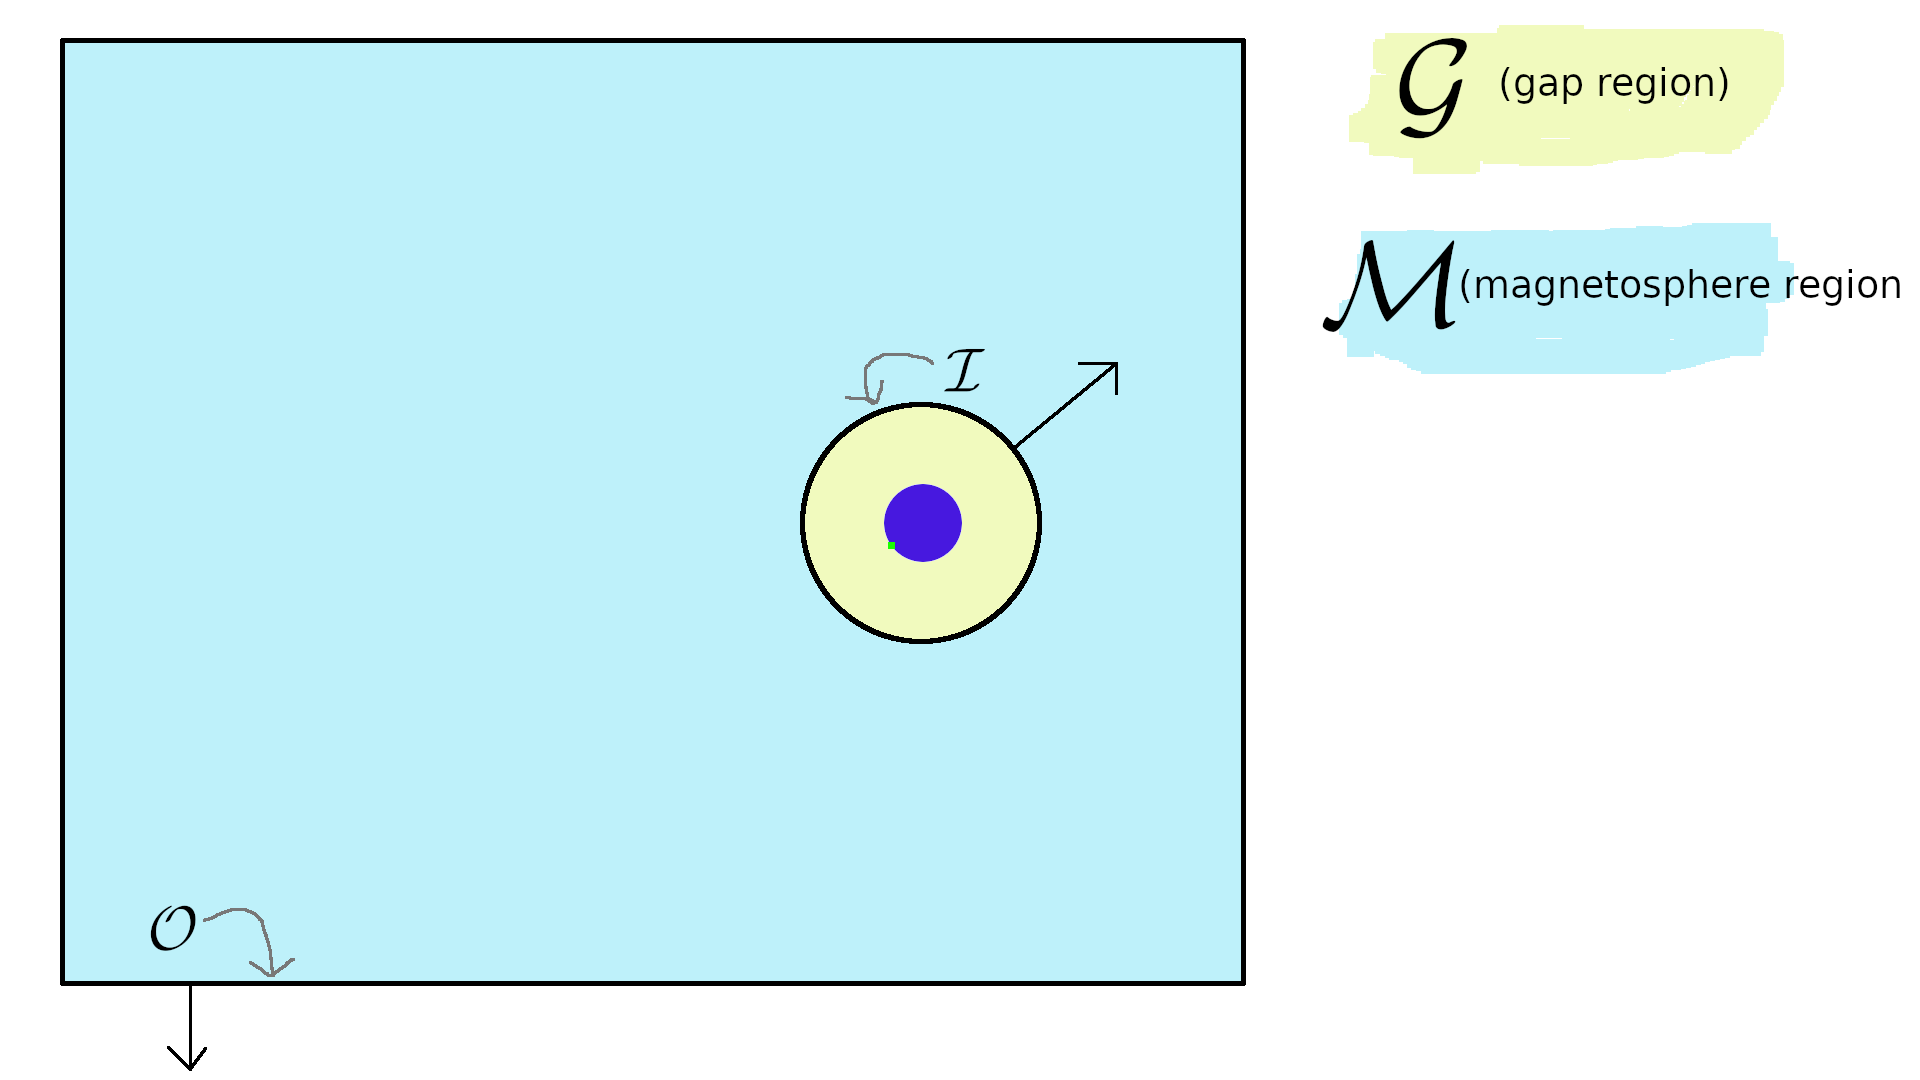
\includegraphics[width=\textwidth]{regions.png}
  \caption{Simulation regions of a typical simulation.
    In the far--Earth region ($\M$) $\B$ is known, and in the near--earth region ($\G$) $\J$ is known.
We also show the outer surface ($\Out$) and the inner surface ($\I$).
    }
  \label{regions}
\end{figure}

MHD (magntohydrodynamics) solvers work by iterating through a few fundamental variables in their domain, and expressing everything else in terms of those variables \citep{Ledvina2008}. The magnetic field $\mathbf{B}$ is a fundamental variable, and the current $\mathbf{J}$ is derived as $\mathbf{J} = \boldsymbol{\nabla} \times \mathbf{B}/\mu_0$. Note we are ignoring displacement current (${\partial \mathbf{E}}/{\partial t}$) here, an assumption that is common in magnetosphere MHD simulations.

There are several models of the magnetosphere which utilize MHD to model the the dynamics of the solar wind in the magnetosphere.
These models typically couple with other types of models that better capture near--Earth dynamics (ionosphere, ring current).
These coupled models have been used to predict geomagnetic perturbations on Earth's surface.
The simulation domains are shown in Figure \ref{regions}. Inside of
the near--Earth region, ($\G$), $\J$ is known and we typically do not have access to $\B$ directly.
In this paper, we investigate methods for computing $\B$ and also examine their consistency.

Inside the near--Earth region, ($\G$), we have direct access to $\J$ and so we could calculate its contribution to $\B$ inside $\G$ using the Biot--Savart integral.

The question becomes how to calculate the contribution of $\mathcal{M}$ to $\mathbf{B}$ inside $\G$.
One method is to use $\mathbf{B}$ from the MHD domain ($\mathcal{M}$), which is known because it is a fundamental variable,
to compute $\mathbf{J} = \boldsymbol{\nabla} \times \mathbf{B}/\mu_0$ inside $\mathcal{M}$.
Then, this $\J$ can be used in a Biot--Savart integral over the far--Earth region $\mathcal{M}$.

This has a few downsides.
In this scenario, $\mathbf{B}$ is calculated solely via Biot--Savart over electric currents,
and only over $\mathcal{G} \cup \mathcal{M}$.
This immediately raises the question
``what about currents outside the simulation volume?''.
This method ignores them, and has no way of evaluating their contribution to surface $\B$.
This could potentially ignore important effects,
like a long distance IMF (interplanetary magnetic field)
due to currents spanning thousands of $R_E$.
A further concern is that $\boldsymbol{\nabla} \boldsymbol{\cdot} \B = 0$ is assumed in the derivation of the Biot-Savart integral from $\mathbf{J} = \boldsymbol{\nabla} \times \mathbf{B}/\mu_0$ and not all MHD solvers will produce $\B$ such that $\boldsymbol{\nabla} \boldsymbol{\cdot} \B = 0$.

Alternative, and we argue better,
methods can be constructed utilizing the Helmholtz Decomposition Theorem (HDT),
which is a general mathematical statement about vector fields from which the Biot--Savart law can be derived with further assumptions.
Some space weather models, such as SWMF, can already implement this approach,
however SWMF does not do so by default (\textbf{is it actually currenntly availabe}).

One thing to note now is that
these other methods for computing $\B$ in some sense already assume there exists a well defined magnetic field throughout the entire simulation volume ($\G \cup \M$).
By utilize the HDT to reconstruct the magnetic field for points within the MhD domain ($\M$), we can apply consistency check on the $\J$ in $\G$ with the $\B$ in $\M$.

In Section \ref{TheoremApplied}, we will discuss how these surface calculations and reconstructions using HDT come about,
after a brief review of the HDT in Section \ref{Theorem}.
Finally in setion \ref{computations} we will show an example of computations done on a SWMF run.

\section{Helmholtz Decomposition Theorem} \label{Theorem}

Before preceding, lets discuss the notation we will use.
(At the moment this isn't precise).
We will denote the set of sufficiently smooth functions as on a region of space $M$ as $\sm{M}$. I.E.

\begin{align}
  \sm{M} &= \left\{ f:M \to \mathbb{R} \, \middle| \, f \text{ is sufficiently smooth} \right\} \nonumber
\end{align}

Similarly, we will denote the set of sufficiently smooth vector fields as $\vsm{M}$.
We will denote the boundary of any such $M$ as $\partial M$.

The Helmholtz Decomposition Theorem \citep{arfken2005mathematical} states that any sufficiently smooth vector field $\mathbf{B}$ in a volume $\Omega$ can be decomposed into the sum of a gradient of a scalar potential $\Phi$ and the curl of a vector potential $\mathbf{A}$: 
\begin{align}
\mathbf{B}&=-\boldsymbol{\nabla}\Phi+\boldsymbol{\nabla}\times\mathbf{A} \label{B_decomp}
\end{align}

where $\forall \x_0 \in \Omega$

\begin{align}
\Phi(\mathbf{x}_0) & =\frac 1 {4\pi} \int_{\Omega} \frac{\boldsymbol{\nabla}\boldsymbol{\cdot}\mathbf{B} (\mathbf{x})}{|\mathbf{x}_0 -\mathbf{x}|} \, \mathrm{d}^3\mathbf{x} -\frac 1 {4\pi} \oint_{\partial \Omega} \mathbf{\hat{n}}_{\partial \Omega} \boldsymbol{\cdot} \frac{\mathbf{B} (\mathbf{x})}{|\mathbf{x}_0-\mathbf{x}|} \, \mathrm{d}S\,, \label{Phi_def} \\[8pt]
\mathbf{A}(\mathbf{x}_0) & =\frac 1 {4\pi} \int_{\Omega} \frac{\boldsymbol{\nabla} \times \mathbf{B}(\mathbf{x})}{|\mathbf{x}_0-\mathbf{x}|} \, \mathrm{d}^3\mathbf{x} -\frac 1 {4\pi} \oint_{\partial \Omega} \mathbf{\hat{n}}_{\partial \Omega}\times\frac{\mathbf{B} (\mathbf{x})}{|\mathbf{x}_0-\mathbf{x}|} \, \mathrm{d}S\,, \label{A_def}
\end{align}

$\partial \Omega$ is the surface that bounds $\Omega$,
and $\mathbf{\hat{n}}_{\partial \Omega}$ is the outward--pointing normal vector on the surface of $\Omega$.

The main result here is the decomposition of a vector field into the sum of an irrotational (curl-free) vector field and a solenoidal (divergence-free) vector field. I.E.
\begin{align}
  \forall \B \in \vsm{\Omega}, \exists \Phi \in \sm{M}, \mathbf{A} \in \vsm{\Omega} :
    \B&=-\boldsymbol{\nabla}\Phi+\boldsymbol{\nabla}\times\mathbf{A} \nonumber
\end{align}
However we also get an integral identity for $\B$ by taking the gradient of Eqn.~\ref{Phi_def} and the curl of Eqn.~\ref{A_def} with respect to $\x_0$.
The derivatives with respect to $\x_0$ can be moved inside the integrals and then substituted into Eqn.~\ref{B_decomp} to yield $\forall \B \in \vsm{\Omega}$,

\begin{align}
\forall \mathbf{x}_0 \in \Omega \label{first_lemma} \\
\mathbf{B}(\mathbf{x}_0) &= \coulombInt{\Omega} \nonumber \\
                                                 &+ \biotsavInt{\Omega} \nonumber \\
                                                 &- \surfInt{\partial \Omega}  \nonumber
\end{align}

There is also a complimentary integral identity for points outside $\Omega$:

\begin{align}
\forall \mathbf{x}_0 \notin \Omega \label{second_lemma} \\
0 &= \coulombInt{\Omega} \nonumber \\
                                                 &+ \biotsavInt{\Omega} \nonumber \\
                                                 &- \surfInt{\partial \Omega}  \nonumber
\end{align}

%Note that the HDT does \textit{not} guarantee the existence of a $\B \in \vsm{\Omega}$ given a $\tilde{\B} \in \vsm{\partial \Omega}$. This issue is discussed in the following section.

\section{Helmholtz Decomposition theorem applied to magnetosphere simulation} \label{TheoremApplied}

In the previous section stands on its own, regardless of any physical interpretation of $\B$.
We chose that variable name with forsight, however, because in this section we will consider $\B$ to represent the magnetic field.
As in the introduction, consider the regions shown in Figure~\ref{regions}.
As discussed, we know the magnetic field on $\M$.
Strictly speaking, we only know it on some discrete set of points in $\M$,
but we use think of it as modeling some smooth function on $\M$.
For example, we can identify derivatives of B with discrete differences and also do numerical integration over $\M$, or some subset of $\M$. \\

So then we have the magnetic field $\B \in \vsm{\M}$.
From this we can in principle compute the relevant integrals for HDT, at least over the integration domain $\M$.
We also have the current density $\mathbf{J}$ in $\mathcal{G}$.
From this we can define and in principle compute:

\begin{align}
  \forall \x_0 \in \GcupM, \B_{\G}(\x_0) := \biotsavIntJ{\G}
\end{align}

Let us now present the full definitions of our Methods outlined in the abstract:

\begin{align}
\forall \mathbf{x}_0 \in \M \\
\B_{\text{MethodA}}(\x_0) &:= \coulombInt{\mathcal{M}} \nonumber \\
            &\qquad + \biotsavInt{\mathcal{M}} \nonumber \\
            &\qquad - \surfInt{\mathcal{O}}  \nonumber \\
            &\qquad + \surfInt{\mathcal{I}}  \nonumber
\end{align}

\begin{align}
\forall \x_0 \in \M \\
  \B_{\text{MethodB}}(\x_0)
        &:= \B_{\G}(\x_0)
          + \coulombInt{\M}
          + \biotsavInt{\M} \nonumber \\
          &\qquad - \surfInt{\Out} \nonumber
\end{align}

\begin{align}
\forall \x_0 \in \G \\
  \B_{\text{Method1}}(\x_0) &:= \B_{\G}(\x_0) \nonumber \\
            &\qquad - \surfInt{\I}  \nonumber
\end{align}

\begin{align}
\forall \x_0 \in \G \\
  \B_{\text{Method2}}(\x_0)
        &:= \B_{\G}(\x_0)
          + \coulombInt{\M}
          + \biotsavInt{\M} \nonumber \\
          &\qquad - \surfInt{\Out} \nonumber
\end{align}

\begin{align}
\forall \x_0 \in \G \\
  \B_{\text{Method3}}(\x_0)
        &:= \B_{\G}(\x_0)
          + \biotsavInt{\M} \nonumber
\end{align}

Note that the expressions for Method B.~and 2.~are identical with the exception that $\x_0$ is in different domains.
All the above integrals are numerically computable with the known output of the MHD simulation.
We expect, up to some numerical integration error, the HDT will hold when it is applicable.

First, we wish to show that HDT (via Eqn~\ref{first_lemma}.) guarentees that Method A.~will reproduce $\B$.
Applying Eqn \ref{first_lemma}.~using $\Omega=\M$ yeilds:

\begin{align}
\forall \x_0 \in \M \nonumber \\
\B(\x_0) &= \coulombInt{\mathcal{M}} \nonumber \\
            &\qquad + \biotsavInt{\mathcal{M}} \nonumber \\
            &\qquad - \surfInt{\partial \mathcal{M}}  \nonumber \\
         &= \coulombInt{\mathcal{M}} \nonumber \\
            &\qquad + \biotsavInt{\mathcal{M}} \nonumber \\
            &\qquad - \surfInt{\mathcal{O}}  \nonumber \\
            &\qquad + \surfInt{\mathcal{I}}  \nonumber \\
         &= \B_{\text{MethodA}}(\x_0)
\end{align}

Here we re-express the surface integral term
by noting $\partial \mathcal{M} = \mathcal{O} \cup \mathcal{I}$
and that $n_{\partial \mathcal{M}} = n_{\mathcal{O}}$ and $n_{\partial \mathcal{M}} = -n_{\mathcal{I}}$ on their respective surfaces.
(see Figure~\ref{regions}.)

Next, we wish to show that HDT (via Eqn~\ref{second_lemma}.) guarentees that Method 1.~and 2.~will agree with each other.
Applying Eqn \ref{second_lemma}.~using $\Omega=\M$ yeilds:

\begin{align}
\forall \x_0 \in \G \nonumber \\
  0 &= \coulombInt{\mathcal{M}} \nonumber \\
            &\qquad + \biotsavInt{\mathcal{M}} \nonumber \\
            &\qquad - \surfInt{\partial \mathcal{M}}  \nonumber \\
         &= \coulombInt{\mathcal{M}} \nonumber \\
            &\qquad + \biotsavInt{\mathcal{M}} \nonumber \\
            &\qquad - \surfInt{\mathcal{O}}  \nonumber \\
            &\qquad + \surfInt{\mathcal{I}}  \nonumber \\
\end{align}

thus

\begin{align}
\forall \x_0 \in \G \nonumber \\
 \B_{\text{Method2}}(\x_0) - \B_{\text{Method1}}(\x_0) &= \B_{\G}(\x_0)
          + \coulombInt{\M}
          + \biotsavInt{\M} \nonumber \\
          &\qquad - \surfInt{\Out} \nonumber \\
          &\qquad -\bigg( \B_{\G}(\x_0) \nonumber \\
            &\qquad \qquad - \surfInt{\I} \bigg) \nonumber \\
         &= \coulombInt{\mathcal{M}} \nonumber \\
            &\qquad + \biotsavInt{\mathcal{M}} \nonumber \\
            &\qquad - \surfInt{\mathcal{O}}  \nonumber \\
            &\qquad + \surfInt{\mathcal{I}}  \nonumber \\
         &= 0
\end{align}

In summary, regardless of what the the simulation outputs,
we expect (up to numerical integration error) that
$\forall \x_0 \in \G, \B_{\text{Method1}}(\x_0) = \B_{\text{Method2}}(\x_0)$ and
$\forall \x_0 \in \M, \B_{\text{MethodA}}(\x_0) = \B(\x_0)$.

Now we wish to go beyond what we can prove using only our $\B \in \vsm{\M}$.

For the results of the simulation to be physically meaningful,
we expect there should exists $\tilde{\B} \in \vsm{\GcupM}$ such that:
$\tilde{\B}|_{\M} = \B$;
$\curl{\tilde{\B}}=\mu_0 \J$ on $\G$; and
$\dive{\tilde{\B}}=0$ on $\G$.
This is not guaranteed for any random 

However, let us now suppose that this is the case.
Then we will show two things.
First, that Methods 1.~and 2.~will actually reproduce said $\tilde{\B}$.
Second, that Method B.~reproduces $\B$.
This last one is important, the mere existence of such a $\tilde{\B}$ guarantees Method B.~reproduces $\B$, where as before we could only show Method A.~rep $\B$. We can use this as a numerical test of how well the models for $\J$ in $\G$ match the MHD values of $\B$ in $\M$.

First, we can apply Eqn~\ref{first_lemma}.~for $\tilde{\B}$ on $\G$

\begin{align}
\forall \x_0 \in \G \\
  \tilde{\B}(\x_0) &= \coulombIntTilde{\G} \nonumber \\
                    &\qquad + \biotsavIntTilde{\G} \nonumber \\
                    &\qquad - \surfIntTilde{\I} \nonumber \\
                   &= 0 + \biotsavIntJ{\G} \nonumber \\
                    &\qquad - \surfInt{\I} \nonumber \\
                   &= \B_{\G}(\x_0) \nonumber \\
                    &\qquad - \surfInt{\I}  \\ \nonumber
                   &= \B_{\text{Method1}}(\x_0)
\end{align}

%Here we first used
%$\tilde{\B}|_{\M} = \B$,
%$\curl{\tilde{\B}}=\mu_0 \J$ on $\G$, and
%$\dive{\tilde{\B}}=0$ on $\G$.
%And then used
%$\partial \mathcal{G} = \mathcal{I}$ and $\mathbf{\hat{n}}_{\partial \mathcal{G}} = \mathbf{\hat{n}}_{\mathcal{I}}$.

Since we already showed $\forall \x_0 \in \G, \B_{\text{Method1}}(\x_0) = \B_{\text{Method2}}(\x_0)$,
it follows

\begin{align}
\forall \x_0 \in \G \\
  \tilde{\B}(\x_0) &= \B_{\text{Method2}}(\x_0)
\end{align}

This can also be obtained by a similarly applying Eqn~\ref{first_lemma}.~for $\tilde{\B}$ on $\GcupM$. Furthermore, doing so will alow us to prove our second claim:

\begin{align}
\forall \x_0 \in \GcupM \\
  \tilde{\B}(\x_0) &= \coulombIntTilde{\GcupM} \nonumber \\
                    &\qquad + \biotsavIntTilde{\GcupM} \nonumber \\
                    &\qquad - \surfIntTilde{\partial \GcupM} \nonumber \\
                   &= \coulombIntTilde{\G} + \coulombIntTilde{\M} \nonumber \\
                    &\qquad + \biotsavIntTilde{\G} + \biotsavIntTilde{\M} \nonumber \\
                    &\qquad - \surfIntTilde{\Out} \nonumber \\
                   &= 0 + \biotsavIntJ{\G} \nonumber \\
                    &\qquad + \coulombInt{\M} + \biotsavInt{\M} \nonumber \\
                    &\qquad - \surfInt{\Out} \nonumber \\
                   &= \B_{\G}(\x_0) \nonumber \\
                    &\qquad + \coulombInt{\M} + \biotsavInt{\M} \nonumber \\
                    &\qquad - \surfInt{\Out} \nonumber \\
                   &=
    \begin{cases}
        \B_{\text{Method2}}(\x_0), & \text{for } \x_0 \in \G \\
        \B_{\text{MethodB}}(\x_0), & \text{for } \x_0 \in \M
    \end{cases}
\end{align}

For $\x_0 \in \G$, this is just our previous result.
For $\x_0 \in \M$, however, we also have by assumption $\forall \x_0 \in \M, \tilde{\B}(\x_0) = \B(\x_0)$.
Thus:

\begin{align}
\forall \x_0 \in \M \\
    \B(\x_0) &= \B_{\text{MethodB}}(\x_0)
\end{align}

\section{Numerical computations using SWMF} \label{computations}

\subsection{Setup}

SWMF magnetosphere runs typically use BATSRUS (Block-Adaptive-Tree-Solarwind-Roe-Upwind-Scheme) coupled to RIM (Ridely Ionosphere Model).
BATSRUS will run an MHD solver in the regions outside of a user defined radius denoted \texttt{rBody}.
However, due to edge effects, the values at \texttt{rBody} are not considered meaningful, and SWMF instead takes the values at a larger user defined radius, denoted \texttt{rCurrents}, in order to generate FAC's coupling the ionosphere to the outer magnetosphere. See \citep{Toth2005}.

If the user requests, SWMF will output it's own datafiles with the `magnetic perturbations' for points on the surface of Earth.
This is really just trying to recreate the surface $\B$ as we discussed.
SWMF breaks the `magnetic perturbation' into 4 contributions:
\texttt{dBMhd}, \texttt{dBFac}, \texttt{dBHal}, \texttt{dBPed}.
\texttt{dBHal} and \texttt{dBPed} are 2D Biot--Savart integrals over the Hall and Pedersen ionosphere currents respectively.
\texttt{dBFac} is the Biot--Savart integral over the field aligned currents, over the region between the ionosphere up to \texttt{rCurrents}.
Thus together, \texttt{dBFac+dBHal+dBPed} is just $\B_{\G}$.
\texttt{dBMhd} is meant to be the contribution from currents outside \texttt{rCurrents}.
\texttt{dBMhd} is calculated in two different ways, based ont the boolean, (\texttt{UseSurfaceIntegrals}), that the user can configure.
If it is \texttt{True}, dBMhd will be calculated
using a surface integral over a sphere of radius \texttt{rCurrents}.
If it is \texttt{False}, dBMhd will be calculated
using a Biot-Savart integral of the current over the
MHD simulation volume, outside of \texttt{rCurrents}.
So effectively,
\texttt{UseSurfaceIntegrals=True} means use Method 1;
\texttt{UseSurfaceIntegrals=False} means use Method 3. See \citep{swmfmanual}

Also, SWMF will output datafiles giving the values of the MhD variables on the block-tree-grid cell centers.
One of these variables is \texttt{b1}: the magnetic field, subtracting out the earths diple.
This is what we used as our $\B$ in $\M$.
Another variable included is \texttt{j}: the current density.
This current density is not an MhD variable, as we discussed before in general.
Instead SWMF simply computes the curl itself (via finite difference) before writing the output file.
We did not use this \texttt{j} anywere, and instead computed $\curl \B$ ourselves from \texttt{b1}.

\subsection{Example}

We show a few SWMF runs as examples. We will look at CARR\_Scenario\_1 (also know as DIPTSUR2) and SWPC\_SWMF\_052811\_2.
These and many other SWMF runs can be found at the CCMC database, see \citep{ccmcdatabase}.
Both of these runs had \texttt{UseSurfaceIntegrals=False}.

First, we will consider the field on the surface of Earth, and take $\x_0$ to be Colaba (geographic latitude=$18.907^\circ$, longitude=$72.815^\circ$).
We wish to verify we can reproduce SWMFs calculation for each run (see Fig \ref{CARRreproduceswmf} and \ref{SWPCreproduceswmf}).
Then we will compare methods 1 2 and 3 (see Fig \ref{CARRcompare123} and \ref{SWPCcompare123}).
Finally, we will the field inside the magnetosphere,
and take $\x_0$ to be (x,y,z)=(0.71875,0.09375,-3.71875) in GSM coordinates in Units of $R_E$.
For brevity lets call this ``GMpoint1".
Then we will compare methods A and B (see Fig \ref{CARRcompareAB} and \ref{SWPCcompareAB}).

\textbf{CARR\_Scenario\_1:}

\begin{figure}[H]
  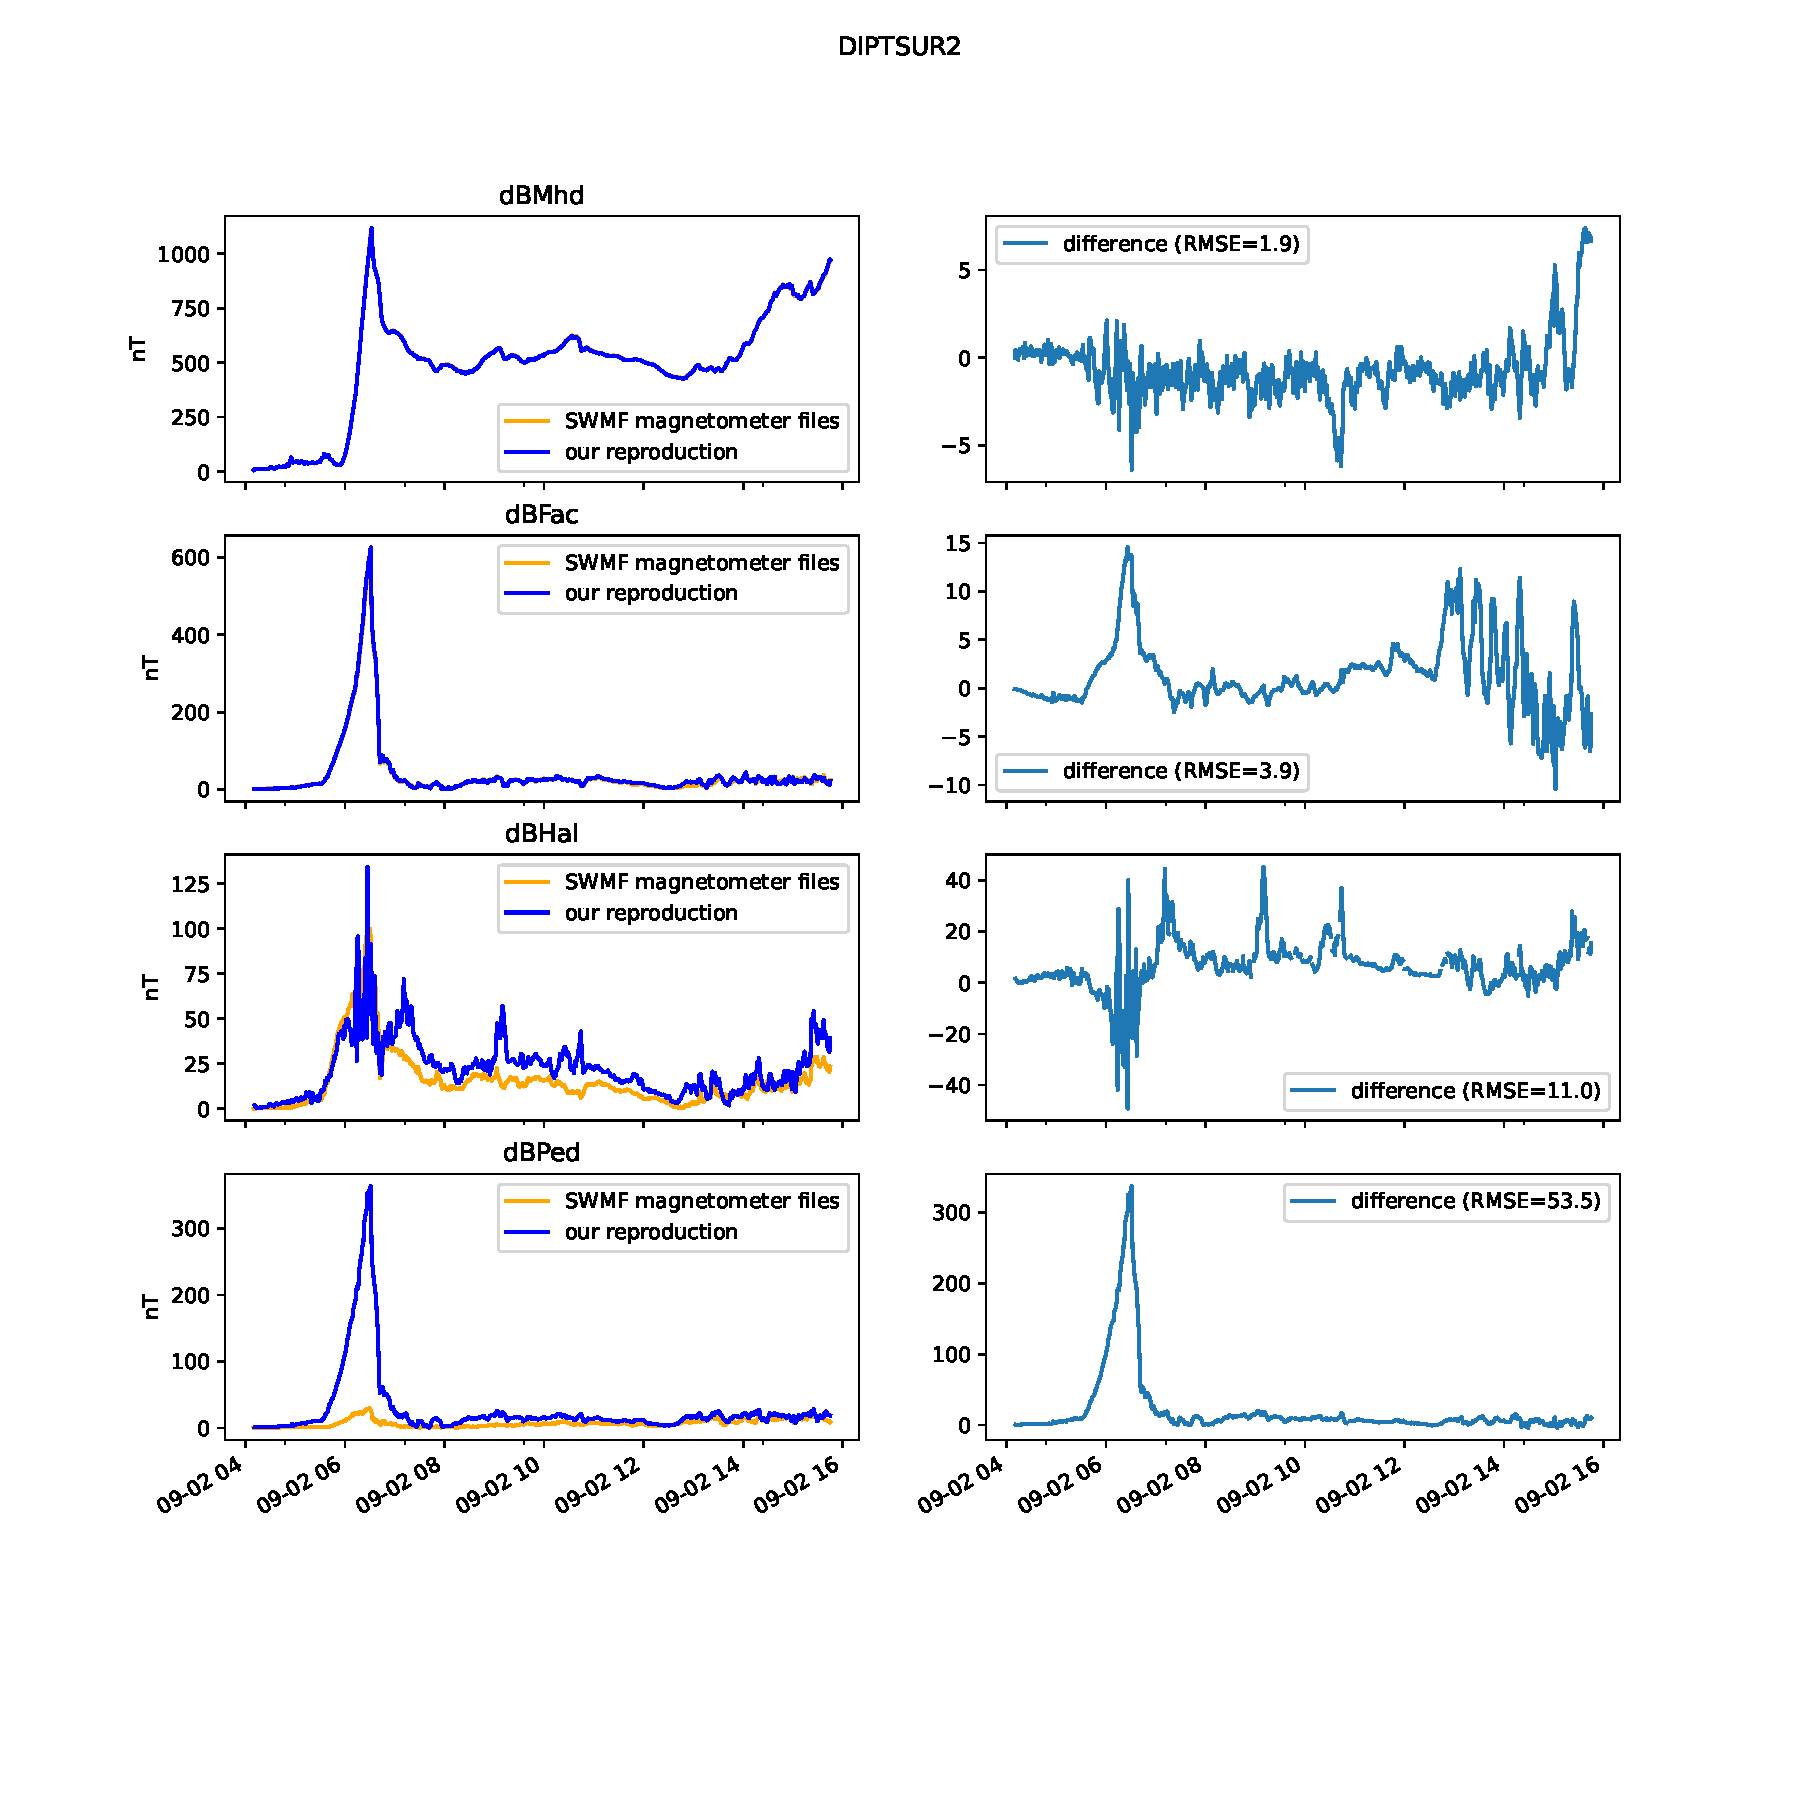
\includegraphics[width=\textwidth]{figures/DIPTSUR2-reproduceswmf.pdf}
  \caption{
  This plot is for CARR\_Scenario\_1.
  Here we plot \texttt{dBMhd}, \texttt{dBFac}, \texttt{dBHal}, \texttt{dBPed},
  which are the SWMF calculations of the `contributions to magnetic perturbations on the ground'. Against it, is our attempts to reproduce SWMF's computations.
  The agreement with RMSE of $1.9$~nT demonstrates that our implementation of the Biot--Savart integration on the BATSRUS grid (as well as our calculation of the curl) reproduces SWMF's computation.
  It also sets a scale for the expected numerical integration error.
  }
  \label{CARRreproduceswmf}
\end{figure}

\begin{figure}[H] 
  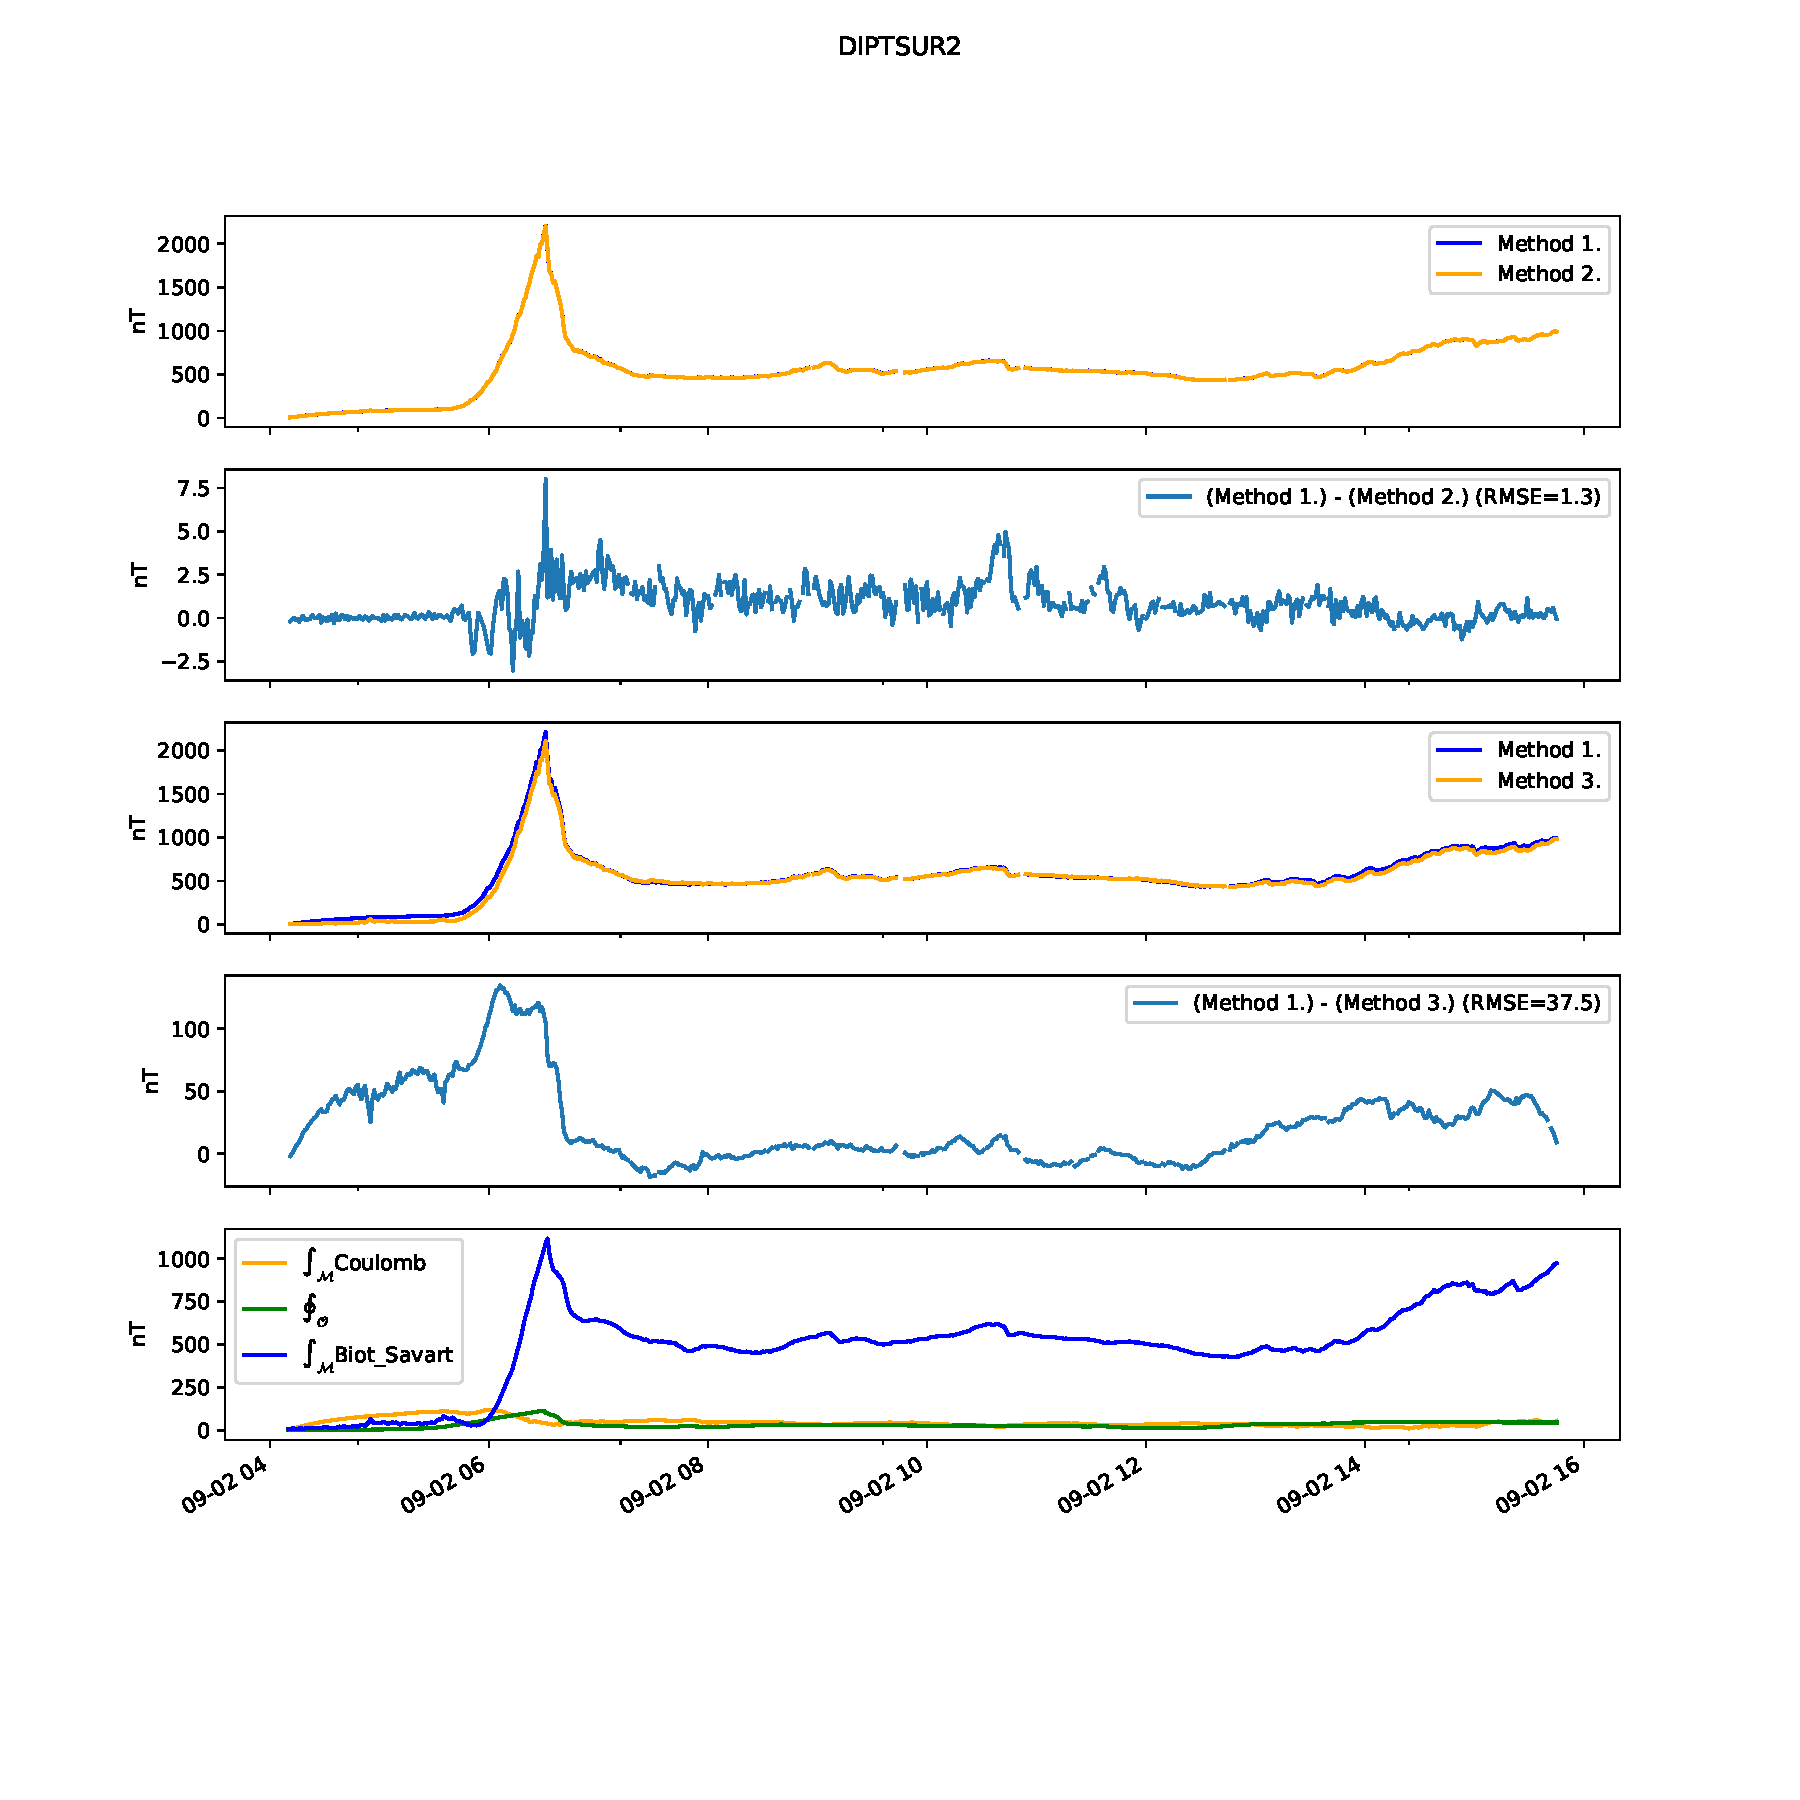
\includegraphics[width=\textwidth]{figures/DIPTSUR2-compare123.pdf}
  \caption{
  This plot is for CARR\_Scenario\_1.
Comparison of Methods (1) and (2) and (3) calculations.
Methods (1) and (2) agree to within the determined scale for the expected numerical integration error.
Method (3), however, does not.
In the lowest plot, we plotted the different terms respnsible for Methods (2) and (3).
It shows the Coulomb term, which can be interpreted as magnetic monopoles, dominates before the spike.
    %Method (2) and (3) have RMSE of $38.7$~nT
  }
  \label{CARRcompare123}
\end{figure}

\begin{figure}[H]
  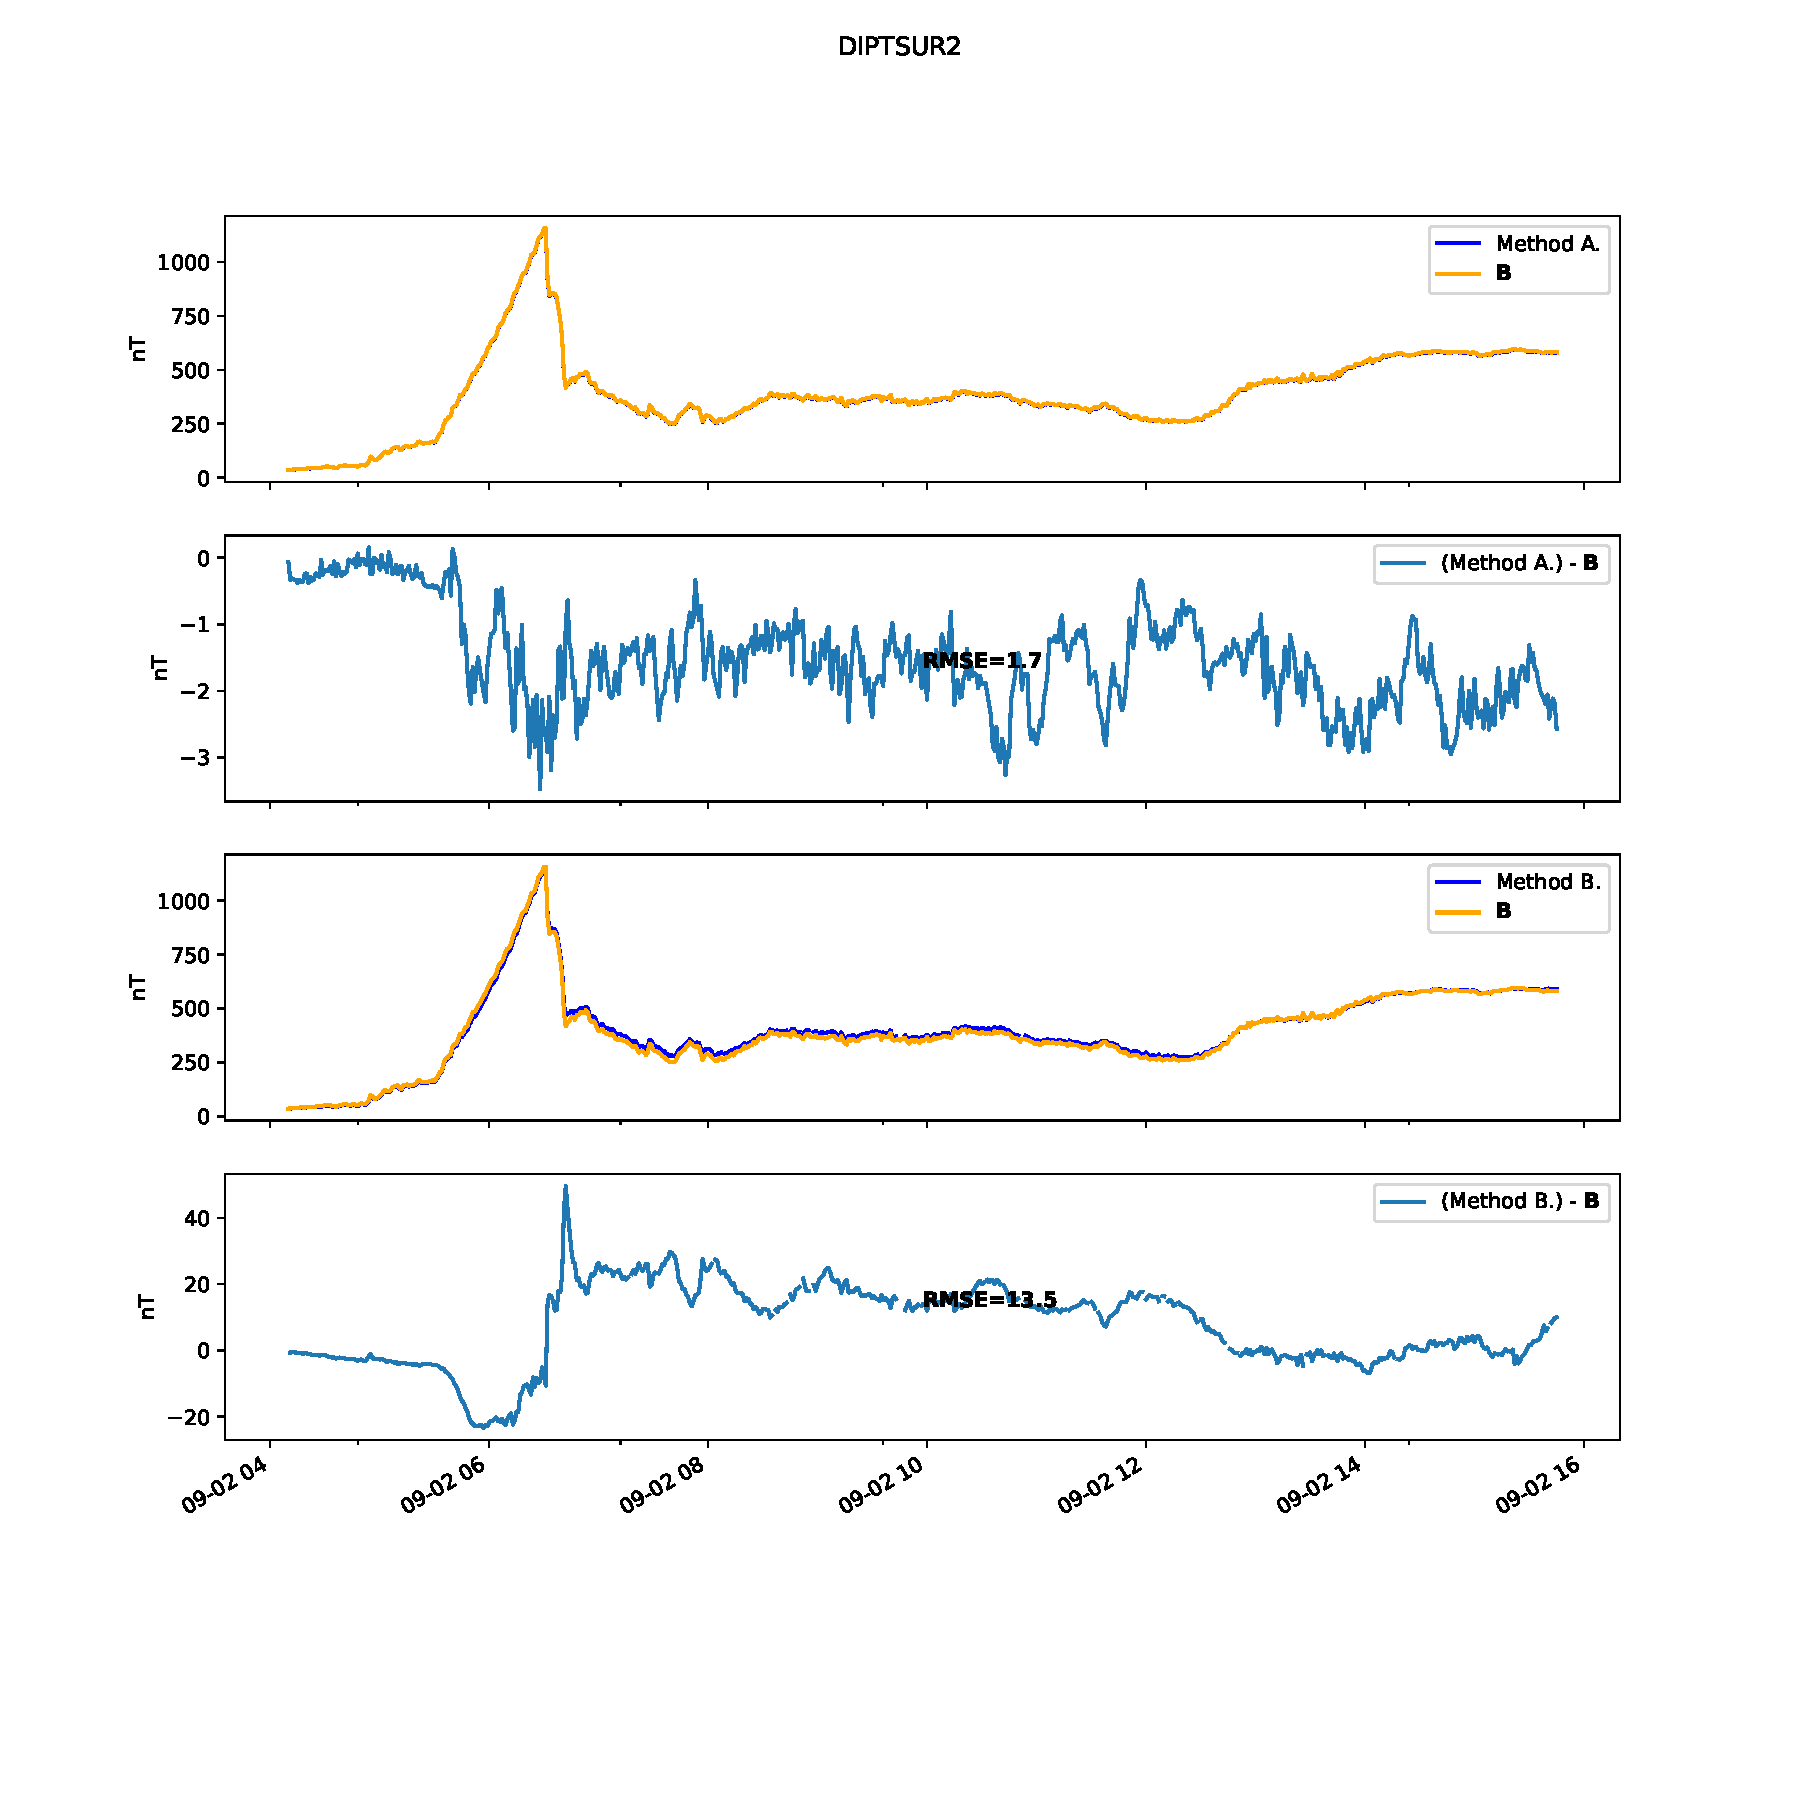
\includegraphics[width=\textwidth]{figures/DIPTSUR2-compareAB.pdf}
  \caption{
  This plot is for CARR\_Scenario\_1.
Shows Method (A) and (B) attempt to reconstruct $\B$.
Method (A) agrees to within the determined scale for the expected numerical integration error.
Method (B) does not.
  }
  \label{CARRcompareAB}
\end{figure}

\begin{figure}[H] 
  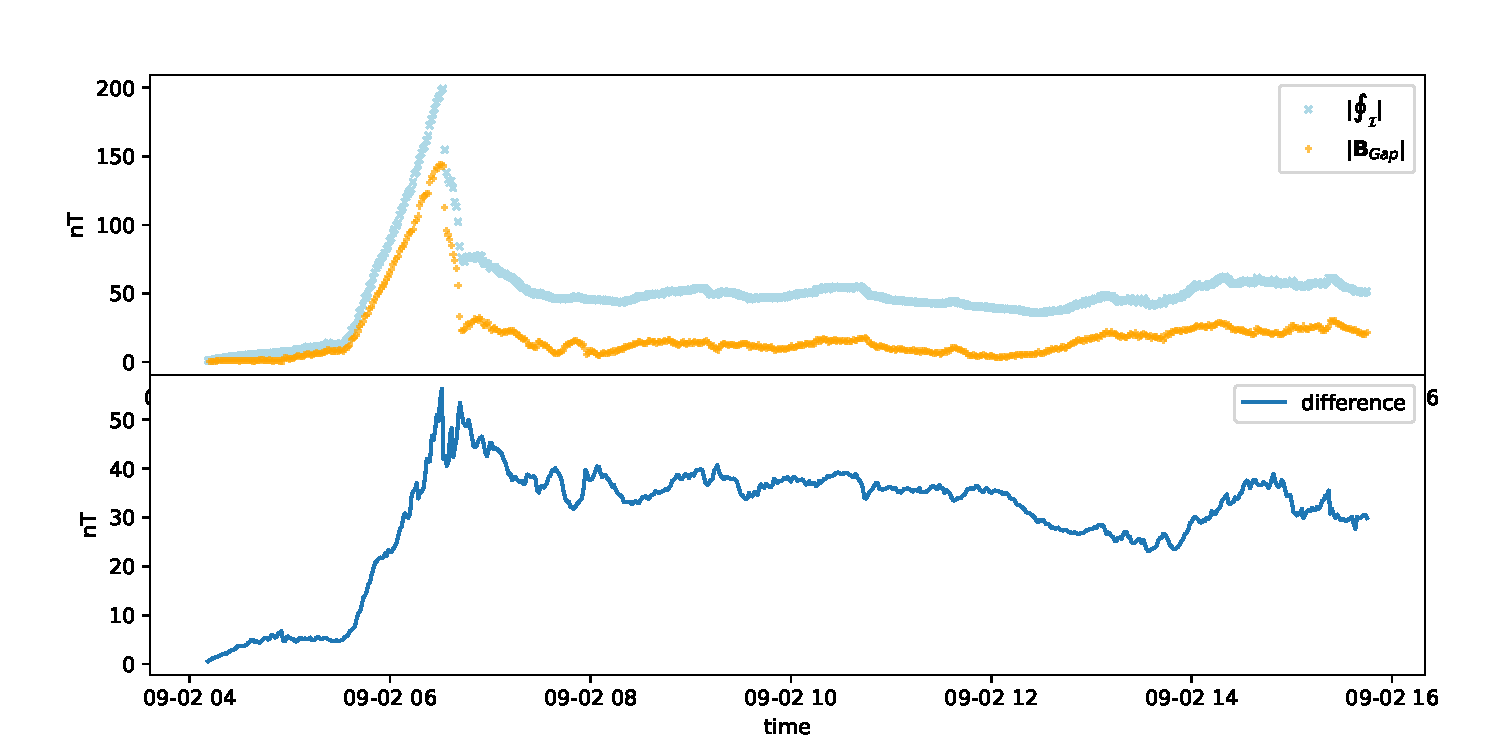
\includegraphics[width=\textwidth]{test_iono_GMpoint1.pdf}
  \caption{
It is important to keep in mind that for this point and run,
the values of $\B_{\G}$ are a relatively small fraction of $\B$.
Upon replotting only $\B_{\G}$ and $\oint_{\I}$,
we obtain a hopefully more direct comparison for the consistancy of the MHD solver with the ionosphere models.
Note $-\B_{\G}$=$\oint_{\I}$ is equivalent to Method(B)=Method(A).
  }
  \label{CARR_conscheck}
\end{figure}

\textbf{SWPC\_SWMF\_052811\_2:}

\begin{figure}[H]
  %\includegraphics[width=\textwidth]{}
  \caption{
  This plot is for SWPC\_SWMF\_052811\_2.
  It is the analogous plots to \ref{CARRreproduceswmf}
  }
  \label{SWPCreproduceswmf}
\end{figure}

\begin{figure}[H]
  %\includegraphics[width=\textwidth]{}
  \caption{
  This plot is for SWPC\_SWMF\_052811\_2.
  It is the analogous plots to \ref{CARRcompare123}
  }
  \label{SWPCcompare123}
\end{figure}

\begin{figure}[H]
  %\includegraphics[width=\textwidth]{}
  \caption{
  This plot is for SWPC\_SWMF\_052811\_2.
  It is the analogous plots to \ref{CARRcompareAB}
  }
  \label{SWPCcompareAB}
\end{figure}

\section{Conclusion}

Ideally the field would have zero divergence everywhere.
In such a case, it wouldn't make sense to only integrate currents over the simulation volume when you can calculates the actual field from *all* currents.

Although utilizing the surface integral method will effectively include contributions from the numerical artifact monopoles, I would argue it is the job of the MHD solver to make sure those are small, it not the job of any postprocessing to ignore it.

Also it is more computationally efficient. Both because it is a surface integral over far less points,
and because it is more direct, in the following sense. The surface integrals
use only B, and not divB or curlB. B is already a fundamental variable of the MHD solver.

%\section{Appendix}
%
%Note we can express the volume Coulomb and Biot-Savart integrals over $\mathcal{M}$ in terms of surface integrals by equating the expressions for $\mathbf{B}(\mathbf{x}_0)$ in Eqn.~\ref{firstBx0} and Eqn.~ \ref{secondBx0} because the $\mathbf{B}_{Gap}(\mathbf{x}_0)$ would cancel out.
%
%We could also derive the same expression using the second lemma, since $\mathbf{x}_0 \notin \mathcal{M}$.
%Because $\partial \mathcal{M} = \mathcal{I} \cup \mathcal{O}$, $\mathbf{\hat{n}}_{\partial \mathcal{M}} = -\mathbf{\hat{n}}_{\mathcal{I}}$ on their respective surfaces.  Also, $\mathbf{\hat{n}}_{\partial \mathcal{M}} = \mathbf{\hat{n}}_{\mathcal{O}}$ by definition.
%
%\begin{align}
% 0  &= \coulombInt{\mathcal{M}}
%     + \biotsavInt{\mathcal{M}}  \\
%    &- \surfInt{\partial \mathcal{M}} \nonumber \\ \nonumber \\
%    &= \coulombInt{\mathcal{M}}
%     + \biotsavInt{\mathcal{M}}  \\
%    &- \surfInt{\mathcal{O}} \nonumber \\
%    &- \surfIntNEG{\mathcal{I}} \nonumber \\ \nonumber \\ 
%    &= \coulombInt{\mathcal{M}}
%     + \biotsavInt{\mathcal{M}}  \\
%    &- \surfInt{\mathcal{O}} \nonumber \\
%    &+ \surfInt{\mathcal{I}} \nonumber
%\end{align}
%
%This can be rearranged to express the volume Coulomb and Biot--Savart integrals over $\mathcal{M}$ in terms of surface integrals.
%
%\begin{align} \label{equalSV}
%  \coulombInt{\mathcal{M}} & +\biotsavInt{\mathcal{M}} =  \\
%    &  \surfInt{\mathcal{O}} \nonumber \\
%     - &\surfInt{\mathcal{I}} \nonumber
%\end{align}

\bibliography{refs}

\end{document}
